\documentclass[12pt, twoside]{article}
\usepackage[letterpaper, margin=1in, head=30pt, headsep=0.1in]{geometry}
\usepackage[english]{babel}
\usepackage[utf8]{inputenc}
\usepackage{amsmath}
\usepackage{amsfonts}
\usepackage{amssymb}
\usepackage{tikz}
%\usetikzlibrary{quotes, angles}

\usepackage{graphicx}
\usepackage{enumitem}
\usepackage{multicol}

%\usepackage{pgfplots}
%\pgfplotsset{width=10cm,compat=1.9}
%\usepgfplotslibrary{statistics}
%\usepackage{pgfplotstable}
%\usepackage{tkz-fct}
%\usepackage{venndiagram}

\usepackage{fancyhdr}
\pagestyle{fancy}
\fancyhf{}
\renewcommand{\headrulewidth}{0pt} % disable the underline of the header
\raggedbottom
\newif\ifmeta
\metatrue %print standards and topics tags

\title{Math AI Worksheet Generator and Formative Assessment System}
\author{Chris Huson}
\date{August 2019}

\fancyhead[RE]{\thepage}
\fancyhead[RO]{\thepage \\ Name: \hspace{3cm}}
%\fancyhead[L]{BECA / Dr. Huson / 10th Grade Geometry\\* 7 June 2019}
%
%\begin{document}
%\subsubsection*{13.7 Homework: Cross sections, distance applications}
\fancyhead[L]{BECA / Dr. Huson / Geometry 02-Midpoint+distance\\* pset ID: 20}

\begin{document}

\subsubsection*{2-4DN-Triangle-area.tex}
\begin{enumerate}
\item Complete the construction of a perpendicular bisector and fill in the blanks in the steps.
      \begin{enumerate}
        \item Given the line segment $\rule{2cm}{0.15mm}$.
        \item Construct circle $A$ with radius $AB$.
        \bigskip
        \item Construct circle $\rule{2cm}{0.15mm}$  with radius $\rule{2cm}{0.15mm}$. 
        \item Label the intersections of the two circles $P$ and $Q$. \bigskip
        \item Draw line $\rule{2cm}{0.15mm}$.
        \item Label the intersection of $\overline{AB}$ and $\overleftrightarrow{PQ}$ as point $M$.
        \item $M$ is the midpoint of $\overline{AB}$ and $\overline{AB} \perp \overleftrightarrow{PQ}$
      \end{enumerate}
      \vspace{7cm}
      \begin{center}
      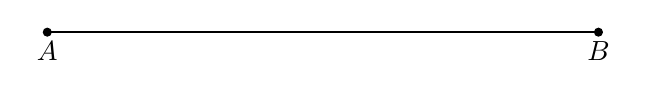
\begin{tikzpicture}
        \draw [-, thick] (0,0)--(7,0);
        \draw [fill] (0,0) circle [radius=0.05] node[below]{$A$};
        \draw [fill] (7,0) circle [radius=0.05] node[below]{$B$};
      \end{tikzpicture}
      \end{center}

\newpage

\item Given the ray $\overrightarrow{AM}$. Mark the point $B$ on $\overrightarrow{AM}$ such that $M$ is the midpoint of $\overline{AB}$,  that is, $\overline{AM} \cong \overline{BM}$.\\[0.75cm]
  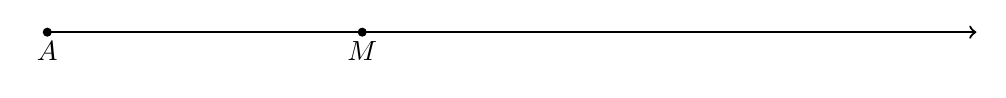
\begin{tikzpicture}
    \draw [->, thick] (0,0)--(11.8,0);
    \draw [fill] (0,0) circle [radius=0.05] node[below]{$A$};
    %\draw [fill] (11.8,0) circle [radius=0.05] node[below]{$B$};
    \draw [fill] (4,0) circle [radius=0.05] node[below]{$M$};
  \end{tikzpicture}
\vspace{1cm}

\item Find the area of $\triangle ABC$. The altitude $h$ of the triangle is 3.75 centimeters and the base $AB=8.4$ cm.\\[0.5cm]
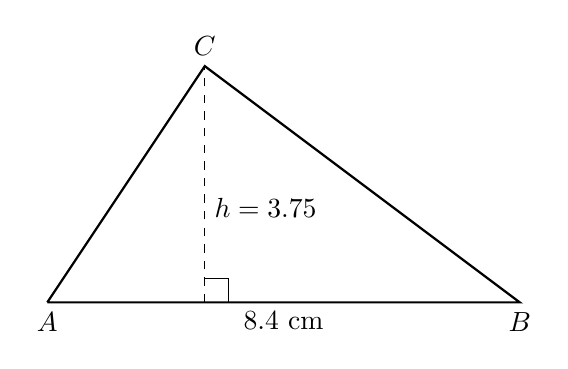
\begin{tikzpicture}[scale=1]
  \draw [thick]
    (2,0)node[below]{$A$}--
    (8,0)node[below]{$B$}--
    (4,3)node[above]{$C$} --(2,0);
 \draw [dashed] (4,0)--(4,3);
 \draw (4,0)++(0.3,0)--++(0,0.3)--+(-0.3,0);
 \node at (4,1.2)[right]{$h=3.75$};
 \node at (5,0)[below]{$8.4$ cm};
\end{tikzpicture} \vspace{1.0cm}


\item Given $\overline{PQR}$, with $PQ=2x-5$, $QR=x+3$, and $PR=19$. Find ${x}$.\\
Complete all the steps for full credit. \smallskip


\vspace{4cm}

\item Given that $Q$ bisects $\overline{PR}$. $PQ=2x-5$, $QR=x+3$. Find ${x}$.\\
Complete all the steps for full credit.

\end{enumerate}
\end{document}